% https://zhuanlan.zhihu.com/p/1934063947264292425
\documentclass[tikz,margin=1cm]{standalone}
\usepackage{tikz-3dplot}
\usepackage{xcolor}
\newcommand{\pla}[2]{%
    \begin{scope}[tdplot_main_coords,#1]
        \foreach \col[count=\n] in {#2} {
            \pgfmathsetmacro{\x}{mod(\n-1,3)-1.5}
            \pgfmathsetmacro{\y}{(\n-\x-7)/3}
            \filldraw[
                line width=2pt,
                draw=black,fill=\col,
                rounded corners=5pt
            ] (-\x,-\y)--++(-1,0)--++(0,-1)--++(1,0)--cycle;
        }%
    \end{scope}
}
\begin{document}
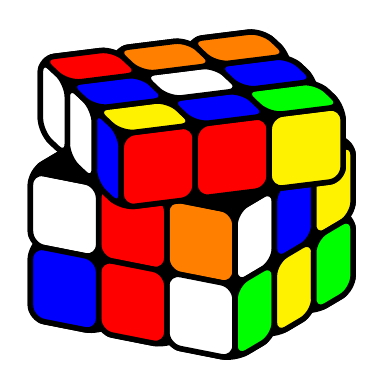
\begin{tikzpicture}
    \pgfmathsetmacro{\xrot}{70}
    \pgfmathsetmacro{\zrot}{120}
    \tdplotsetmaincoords{\xrot}{\zrot}
    \pla{canvas is yz plane at x=-1.5,yshift=-1cm}{,,,,,}
    \pla{canvas is xz plane at y=-1.5,yshift=-1cm}{,,,,,}
    \pla{canvas is xy plane at z=-1.5}{,,,,,,,,}
    \pla{canvas is yz plane at x=1.5,yshift=-1cm}{orange,red,white,white,red,blue}
    \pla{canvas is xz plane at y=1.5,yshift=-1cm}{white,blue,yellow,green,yellow,green}
    \pla{canvas is xy plane at z=0.5}{,,,,,,,,}
    \pgfmathsetmacro{\zrot}{160} % 旋转
    \tdplotsetmaincoords{\xrot}{\zrot}
    \pla{canvas is yz plane at x=-1.5}{,,}
    \pla{canvas is xz plane at y=-1.5}{,,}
    \pla{canvas is xy plane at z=0.5}{,,,,,,,,}
    \pla{canvas is yz plane at x=1.5}{blue,white,white}
    \pla{canvas is xz plane at y=1.5}{red,red,yellow}
    \pla{canvas is xy plane at z=1.5}{yellow,blue,green,blue,white,blue,red,orange,orange}
\end{tikzpicture}
\end{document}